\section{Dark Matter Searches}
\par
Maybe have this as a separate chapter? And go into more detail about signals?

\par
There are generally speaking, three routes of detection can be classified as;

\begin{itemize}
    \item Production
    \item Indirect
    \item Direct
\end{itemize}
    
    

\subsection{Direct Detection}

\begin{figure}[!htbp]%
    \centering
    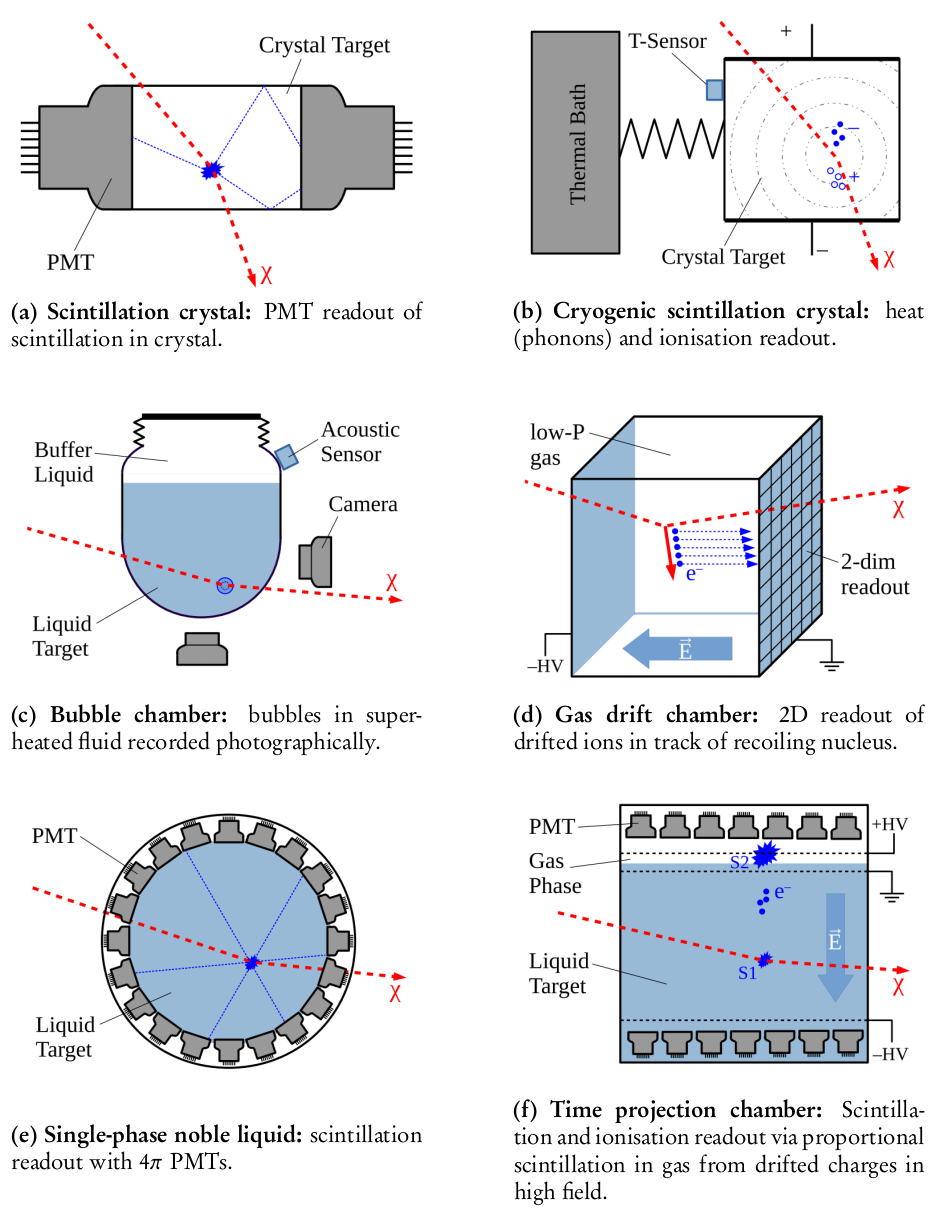
\includegraphics[width=0.8\textwidth]{Figures/DarkMatterEvidence/direct_detection_methods.png}
    \caption[Schematics of signal readouts from direct detectors]{test}
    \label{fig:SearchMethods_Direct_Detection}
\end{figure}

\subsection{Indirect Detection}

\par
Among some of the most exciting results of this so far are from a $\gamma$-ray excess from the galactic centre.
Two theories persist to account for this, namely dark matter annihilation \cite{galactic_gamma_excess_1_ref, galactic_gamma_excess_2_ref}, or millisecond pulsars \cite{galactic_gamma_excess_3_ref, galactic_gamma_excess_4_ref}.

\par
Though recently some doubt has been cast over the template fitting method used, indicating that even if the signal source was dark matter, it would not have been detected \cite{galactic_gamma_excess_5_ref}.
Leaving there to be much 


\subsection{Production}
\par
In some experiments it may be possible to produce dark matter.
In particle colliders such as the Large Hadron Collider (LHC) this process may occur.
The act of smashing together protons and observing the jets output.
This may occur in proton-proton collisions: $pp\xrightarrow{}\chi\chi$.

\par
When two protons are collided together, what is observed are a bunch of jets. 
But we don't care about that... Down with the LHC!

\par
The primary observable applicable to a dark matter search is the missing momentum.
A search may be performed by searching for an excess of this missing energy when compared to the Standard Model background.





\par
Though these experiments may not be able to fully characterise dark matter, they do offer the best way for discovering new invisible particles.
However, they are hindered as any dark matter particle mass to be approximately 50\% of the mediator mass.
Though this is complimented by what direct detection offers with the sensitivity limited by the neutrino
\par
The LHC, at the time of writing, is undergoing an upgrade ahead of a planned 14 TeV centre-of-mass energy science run. 
This High-Luminosity run, due to begin data-taking in 2026 will allow for improved searches into dark matter.

